\documentclass{article}
\usepackage[utf8]{inputenc}
\usepackage{hyperref}
\usepackage{graphicx}

\title{NLP Project Proposal}
\author{Andreas Kuster, Viswa Virinchi, Jakub Filipek}
\date{\today}

\begin{document}

\maketitle

\section*{Citation}

Title: ner and pos when nothing is capitalized \\

\noindent
Url: \href{https://www.aclweb.org/anthology/D19-1650/}{www.aclweb.org/anthology/D19-1650/} \\

\noindent
Authors: Stephen Mayhew, Tatiana Tsygankova, Dan Roth \\

\noindent
Abstract:  \\
For those languages which use it, capitalization is an important signal for the fundamental NLP tasks of Named Entity Recognition (NER) and Part of Speech (POS) tagging. In fact, it is such a strong signal that model performance on these tasks drops sharply in common lowercased scenarios, such as noisy web text or machine translation outputs. In this work, we perform a systematic analysis of solutions to this problem, modifying only the casing of the train or test data using lowercasing and truecasing methods. While prior work and first impressions might suggest training a caseless model, or using a truecaser at test time, we show that the most effective strategy is a concatenation of cased and lowercased training data, producing a single model with high performance on both cased and uncased text. As shown in our experiments, this result holds across tasks and input representations. Finally, we show that our proposed solution gives an 8\% F1 improvement in mention detection on noisy out-of-domain Twitter data.


\section{Contributions}

\subsection*{Exercise 1a}
TODO: A clear list of the scientific hypotheses evaluated in the original paper. Some papers don't make this super clear, so it can take a couple readings of the paper to understand.


\section{Access to data}
Task: Give a short description of whether and how you can access the data used in the paper.
\\
\\
We can access all the data CoNLL 2003, Penn Treebank and Twitter, but have to do some processing (i.e. cased/uncased/..). The links to the sources are below each F1 score comparison table.


\subsection*{Evaluation 1}
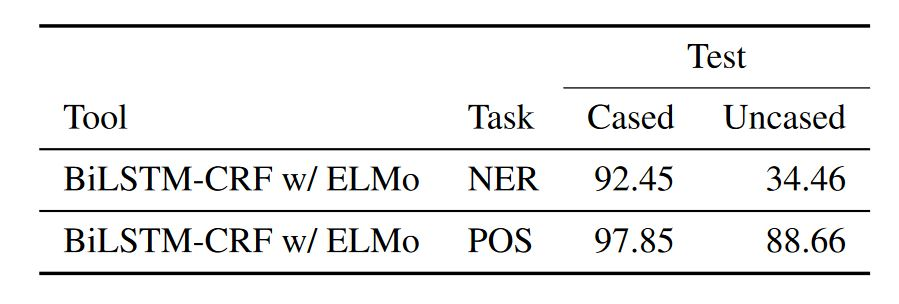
\includegraphics{stat1}
\\
\href{https://dl.acm.org/doi/10.3115/1119176.1119195}{CoNLL}
\\
PTB sections 22-24 \href{https://www.seas.upenn.edu/~pdtb/}{Penn Treebank}


\subsection*{Evaluation 2}
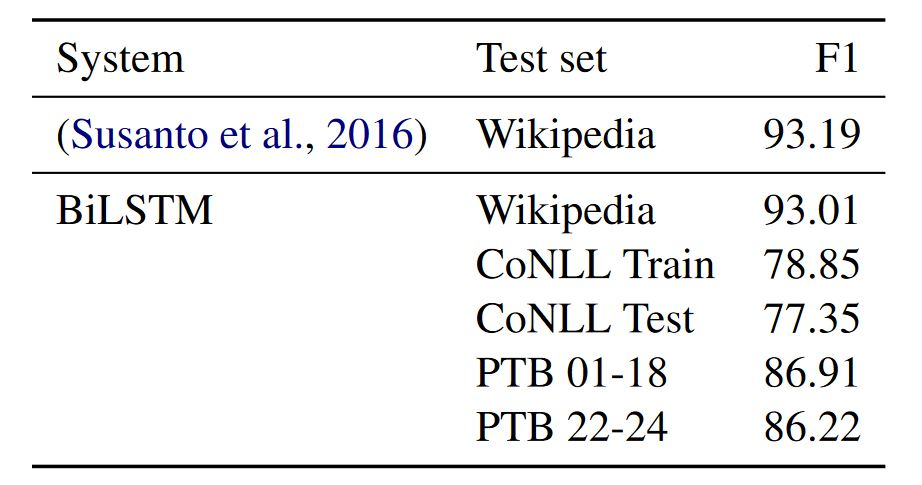
\includegraphics{stat2}

\noindent
\href{https://www.aclweb.org/anthology/W11-1601.pdf}{Wikipedia}\\
\href{https://dl.acm.org/doi/10.3115/1119176.1119195}{CoNLL}\\
PTB sections 22-24 \href{https://www.seas.upenn.edu/~pdtb/}{Penn Treebank}



\subsection*{Evaluation 3}
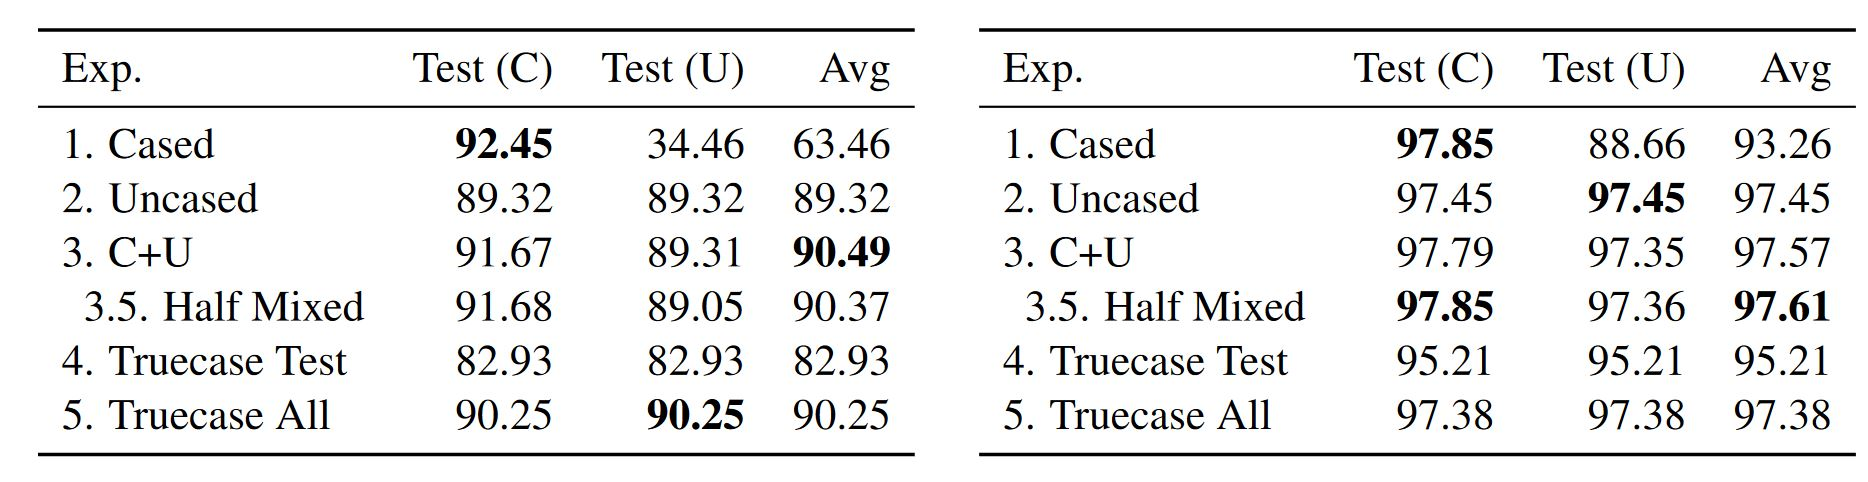
\includegraphics{stat3}

\noindent
\href{https://dl.acm.org/doi/10.3115/1119176.1119195}{CoNLL}\\
PTB sections 22-24 \href{https://www.seas.upenn.edu/~pdtb/}{Penn Treebank}


\subsection*{Evaluation 4}
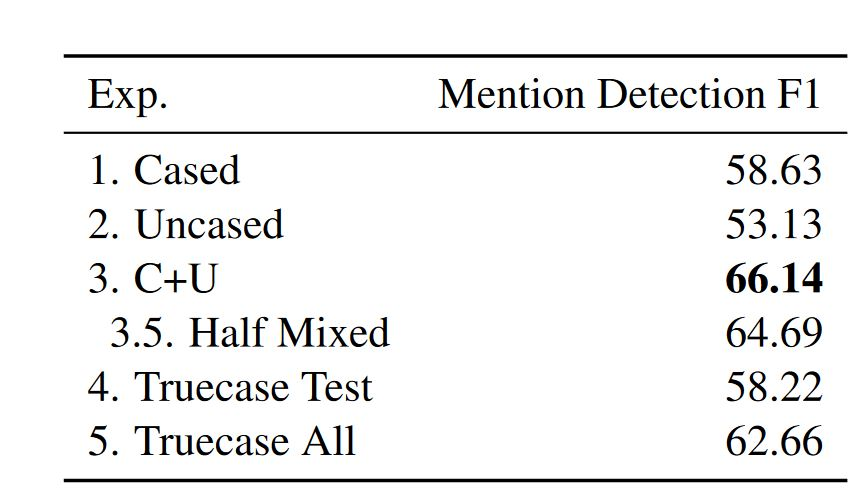
\includegraphics{stat4}
\href{https://github.com/GateNLP/broad_twitter_corpus}{Twitter}




\section{Feasibility}
TODO: a discussion of the feasibility of the computation you will need to do (essentially, an argument that the project will be feasible)



\end{document}
